\documentclass[conference, a4paper]{IEEEtran}

% used for flow charts
\usepackage{tikz}
% FIXME finally no todos should exist in this draft
\usepackage[textsize=tiny]{todonotes}
% positioning is used for below lef = of
\usetikzlibrary{shapes,arrows, positioning}

\tikzstyle{vertex}=[circle,fill=black!15,minimum size=10pt,inner sep=0pt, font=\tiny]
\tikzstyle{fifo}=[->]
\tikzstyle{syncdrain}=[>-<]


\title{Active Learning : From Blackbox To Timed Connectors}
\author{
\IEEEauthorblockN{Yi Li\IEEEauthorrefmark{1} and Meng Sun\IEEEauthorrefmark{1}}
\IEEEauthorblockA{
  \IEEEauthorrefmark{1}DI, School of Mathematical Sciences, Peking University,
  Beijing, China\\
  liyi\_math@pku.edu.cn, summeng@math.pku.edu.cn
}
}

\begin{document}
\maketitle
\begin{abstract}
  Coordination is becoming more and more important, especially in concurrent programming and
  distributed systems. More and more tools are built to verify coordination models while most of
  them are facing the same problem: \emph{lack of models}. In many cases, somehow we need to check a
  connector with nothing more than a binary file. In this paper, we present a learning-based
  framework to formally verify a Reo connector in case there is no source code. From some practical
  cases, we've shown the effciency of our approach. Both the algorithm and Reo itself have been
  ported to \emph{Golang}, making it fully-prepared for parallel programming.
\end{abstract}

\begin{IEEEkeywords}
  active learning, coordination, formal method.
\end{IEEEkeywords}

\section{Introduction}

In the past few years, researchers have been focusing on this area, and come up with a
series of impressive works. 
\todo{a list}
However, most of these works are based on models, instead of binaries. Then it comes a well-known
problem: \emph{how can we obtain these models?}

The application of machine learning in formal models has a long history. There are several main
orientations: extraction of formal models and learning-guided verification technique.

% it seems that we need a graph to describe how we're doing this work
\todo{better graph}
% Define block styles
\tikzstyle{block} = [rectangle, draw, fill=blue!20, 
text width=4em, text centered, rounded corners, minimum height=3em]
\tikzstyle{line} = [draw, -latex']
\tikzstyle{cloud} = [draw, ellipse,fill=red!20, minimum height=2em, node distance = 2.5cm]

\begin{figure}[h]
  \centering
  \begin{tikzpicture}[node distance = 1.5cm, auto]
    % Place nodes
    \node [block] (reomodel) {REO Models};
    \node [cloud, left of=reomodel] (human) {Human};
    \node [block, below left = of reomodel] (tsamodel) {TSA};
    \node [block, below right = of reomodel] (mealymodel) {Mealy Machines};
    %\node [cloud, left = of tsamodel] (verification) {Verification};
    %\node [cloud, right = of mealymodel] (blackbox) {Blackbox};
    % Draw edges
    \path [line] (reomodel) -- (tsamodel);
    \path [line] (reomodel) -- (mealymodel);
    %\path [line] (tsamodel) -- (evaluate);
    \path [line] (mealymodel) -- (tsamodel);
    \path [line] (mealymodel) |-  (reomodel);
    %\path [line] (update) |- (tsamodel);
    %\path [line] (decide) -- node {no}(stop);
    %\path [line,dashed] (human) -- (reomodel);
  \end{tikzpicture}
  \caption{Our Idea}
  \label{fig:idea}
\end{figure}


In this paper, we presented an adapted active learning algorithm to extract timed Reo connectors
from binaries with no source code needed.

\section{Preliminaries}

\subsection{Reo Coordination Language}
\label{sec:reo}

\subsection{Active Learning and Mealy Machines}

\section{Timed Connectors as Mealy Machines}

Reo Coordination Model, obviously, is not a \emph{proper model} for learning. 

So far as we can tell, most works\cite{DBLP:conf/fase/RaffeltS06} on automata learning are not
capable of infinite models. \todo{reason?} Considering the semantics defined in section
\ref{sec:reo}, it's apparent that every finite connector has a corresponding constraint
automata, and the automata is also finite. Unfortunately, when checking the further definition of
Reo connectors' input, we find that it's not the case.

\todo{an example as graph}
\begin{figure}[h]
\caption{Infinite States in a Reo Model}
\label{fig:reoinfinite}
\end{figure}

While focusing on behavior of connectors, Reo doesn't give detail depiction on behavior of
components. As shown in \figurename \ref{fig:reoinfinite}, connectors are able to reject any datum
if they are not ready. But what will happen outside the connector, if the datum is rejected? This
question deserves careful consideration if we are taking an external view.

\section{From Blackbox to Timed Connectors}
\subsection{Equivalence Query}
Generally, equivalence query has been proved impossible in blackbox
models\cite{DBLP:journals/iandc/Angluin87}. However, in this
section, we're showing that in certain circumstances, equivalence query can be implemented with
no approximation.

Since equivalence queries are used to search for counter-examples, firstly let's see what makes
counter-examples even existing after the \emph{Table Close} algorithm.

\begin{figure}[h]
  \begin{center}
    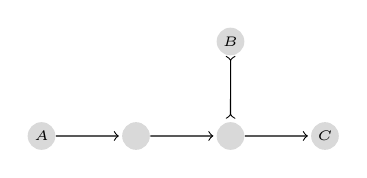
\begin{tikzpicture}[scale=1.2,shorten >=1pt,->]

  \foreach \name/\lbl/\x/\y in {A/A/1/1, B/B/3/2, M1//2/1, M2//3/1, C/C/4/1}
    \node[vertex] (P-\name) at (\x,\y) {$\lbl$};
    
    \draw[fifo] (P-A) -- (P-M1);
    \draw[syncdrain] (P-B) -- (P-M2);
    \draw[fifo] (P-M1) -- (P-M2);
    \draw[fifo] (P-M2) -- (P-C);

\end{tikzpicture}

  \end{center}
  \caption{<+caption text+>}
  \label{fig:buf2}
\end{figure}<++>
\section{Case Studies}

\section{Conclusion and Future Work}



\bibliographystyle{abbrv}
\bibliography{bib}


% FIXME remove this
\listoftodos

\end{document}
